\documentclass[a4paper]{article}
% Some basic packages
\usepackage[utf8]{inputenc}
\usepackage[T1]{fontenc}
\usepackage{textcomp}
\usepackage[english]{babel}
\usepackage{url}
\usepackage{graphicx}
\usepackage{float}
\usepackage{booktabs}
\usepackage{enumitem}
\usepackage{tikz-cd}

\pdfminorversion=7

% Don't indent paragraphs, leave some space between them
\usepackage{parskip}

% Hide page number when page is empty
\usepackage{emptypage}
\usepackage{subcaption}
\usepackage{multicol}
\usepackage{xcolor}

% Math stuff
\usepackage{amsmath, amsfonts, mathtools, amsthm, amssymb}
\usepackage{mathrsfs}
\usepackage{cancel}
\usepackage{bm}
\newcommand\N{\ensuremath{\mathbb{N}}}
\newcommand\R{\ensuremath{\mathbb{R}}}
\newcommand\Z{\ensuremath{\mathbb{Z}}}
\renewcommand\O{\ensuremath{\emptyset}}
\newcommand\Q{\ensuremath{\mathbb{Q}}}
\newcommand\C{\ensuremath{\mathbb{C}}}

\usepackage{systeme}

\let\svlim\lim\def\lim{\svlim\limits}

\let\implies\Rightarrow
\let\impliedby\Leftarrow
\let\iff\Leftrightarrow
\let\epsilon\varepsilon

\usepackage{stmaryrd}
\newcommand\contra{\scalebox{1.5}{$\lightning$}}

\definecolor{correct}{HTML}{009900}
\newcommand\correct[2]{\ensuremath{\:}{\color{red}{#1}}\ensuremath{\to }{\color{correct}{#2}}\ensuremath{\:}}
\newcommand\green[1]{{\color{correct}{#1}}}

\newcommand\hr{
    \noindent\rule[0.5ex]{\linewidth}{0.5pt}
}

\newcommand\hide[1]{}

\usepackage{siunitx}
\sisetup{locale = US}

\usepackage{mdframed}
\mdfsetup{skipabove=1em,skipbelow=0em}
\theoremstyle{definition}
\newmdtheoremenv[nobreak=true]{definition}{Definition}
\newmdtheoremenv[nobreak=true]{property}{Property}
\newmdtheoremenv[nobreak=true]{corollary}{Corollary}
\newmdtheoremenv[nobreak=true]{theorem}{Theorem}
\newmdtheoremenv[nobreak=true]{lemma}{Lemma}
\newmdtheoremenv[nobreak=true]{proposition}{Proposition}

\newtheorem*{example}{Example}
\newtheorem*{notation}{Notation}
\newtheorem*{remark}{Remark}
\newtheorem*{note}{Note}
\newtheorem*{problem}{Problem}
\newtheorem*{observe}{Observe}
\newtheorem*{intuition}{Intuition}
% ... (add other unnumbered theorem-like environments as per your requirement)

\usepackage{etoolbox}
\AtEndEnvironment{example}{\null\hfill$\diamond$}%
% ... (add other environments to end with a diamond if required)

\makeatletter
\def\thm@space@setup{%
  \thm@preskip=\parskip \thm@postskip=0pt
}

\newcommand{\exercise}[1]{%
    \def\@exercise{#1}%
    \subsection*{Exercise #1}
}

\newcommand{\subexercise}[1]{%
    \subsubsection*{Exercise \@exercise.#1}
}

\usepackage{xifthen}
\def\testdateparts#1{\dateparts#1\relax}
\def\dateparts#1 #2 #3 #4 #5\relax{
    \marginpar{\small\textsf{\mbox{#1 #2 #3 #5}}}
}

\def\@lecture{}%
\newcommand{\lecture}[3]{
    \ifthenelse{\isempty{#3}}{%
        \def\@lecture{Lecture #1}%
    }{%
        \def\@lecture{Lecture #1: #3}%
    }%
    \subsection*{\@lecture}
    \marginpar{\small\textsf{\mbox{#2}}}
}

\usepackage{fancyhdr}
\pagestyle{fancy}

\fancyhead[RO,LE]{\@lecture}
\fancyfoot[RO,LE]{\thepage}
\fancyfoot[C]{\leftmark}

\makeatother

\usepackage{todonotes}
\usepackage{tcolorbox}

\tcbuselibrary{breakable}

\newenvironment{correction}{\begin{tcolorbox}[
    arc=0mm,
    colback=white,
    colframe=green!60!black,
    title=Remark,
    fonttitle=\sffamily,
    breakable
]}{\end{tcolorbox}}

\newenvironment{notebox}[1]{\begin{tcolorbox}[
    arc=0mm,
    colback=white,
    colframe=white!60!black,
    title=#1,
    fonttitle=\sffamily,
    breakable
]}{\end{tcolorbox}}

\usepackage{import}
\usepackage{pdfpages}
\usepackage{transparent}
\newcommand{\incfig}[1]{%
    \def\svgwidth{\columnwidth}
    \import{./figures/}{#1.pdf_tex}
}

\pdfsuppresswarningpagegroup=1

\author{Mika Bohinen}

\title{Computational Game Theory \\ Sheet 2 \\
Class Tutor: Mr C. Wang}
\begin{document}
\maketitle

\begin{exercise}{1}
  \begin{enumerate}[label=(\alph*)]
    \item Consider the following payoff matrix for a 2 player game:
      \begin{table}[H]
        \setlength{\extrarowheight}{2pt}
        \centering
        \begin{tabular}{*{4}{c|}}
          \multicolumn{2}{c}{} & \multicolumn{2}{c}{Player $2$}\\\cline{3-4}
          \multicolumn{1}{c}{} &  & $L$  & $R$ \\\cline{2-4}
          \multirow{2}*{Player $1$}  & $T$ & $(1, 1)$ & $(1, 0)$ \\\cline{2-4}
                                     & $B$ & $(1, 1)$ & $(0, -1)$ \\\cline{2-4}
        \end{tabular}
      \end{table}
      Here both $ (T,L) $ and $ (B, L) $ are Nash equilibria, and while $ T $ is a dominant strategy for player 1, $ B $ is not. Hence there is a Nash equilibrium in which a player has not chosen a dominant strategy.

    \item This is false. Simply consider the following payoff matrix:
      \begin{table}[H]
        \setlength{\extrarowheight}{2pt}
        \centering
        \begin{tabular}{*{4}{c|}}
          \multicolumn{2}{c}{} & \multicolumn{2}{c}{Player $2$}\\\cline{3-4}
          \multicolumn{1}{c}{} &  & $L$  & $R$ \\\cline{2-4}
          \multirow{2}*{Player $1$}  & $T$ & $(1, 1)$ & $(1, 1)$ \\\cline{2-4}
                                     & $B$ & $(1, 1)$ & $(1, 1)$ \\\cline{2-4}
        \end{tabular}
      \end{table}
      Here every combination of strategies is a dominant strategy equilibrium. Hence there is no reason for a dominant strategy equilibrium to be unique.

    \item If $ \vec{\sigma} $ is a dominant strategy equilibrium then we must show that there is no $ i \in N $ and $ \sigma'_i \in \Sigma_i $ such that
      \begin{equation*}
        u_i(\vec{\sigma}_{-i}, \sigma'_i) > u_i(\vec{\sigma})
      .\end{equation*}
      This follows directly from the definition of a dominant strategy equilibrium. As if such $ \sigma'_i $ were to exist then it would contradict the assumption that
      \begin{equation*}
        u_i(\vec{\sigma}_{-i}, \sigma_i) \geq u_i(\vec{\sigma}_{-i}, \sigma'_i).
      \end{equation*}

    \item This is not true. To see why, consider the following payoff matrix
      \begin{table}[H]
        \setlength{\extrarowheight}{2pt}
        \centering
        \begin{tabular}{*{4}{c|}}
          \multicolumn{2}{c}{} & \multicolumn{2}{c}{Player $2$}\\\cline{3-4}
          \multicolumn{1}{c}{} &  & $L$  & $R$ \\\cline{2-4}
          \multirow{2}*{Player $1$}  & $T$ & $(-2, -2)$ & $(-3, -3)$ \\\cline{2-4}
                                     & $B$ & $(-3, 0)$ & $(-1, -1)$ \\\cline{2-4}
        \end{tabular}
      \end{table}
      We see that the strategy $ \vec{\sigma} = (T, T) $ is a Nash equilibrium. However, it is not a dominant strategy equilibrium. To see why, suppose player $ Y $ choose $ R $. Then the best response for $ X $ is to choose $ T $. Hence $ X $'s best strategy is dependent upon the strategy $ Y $ chooses which goes against the defining property of a dominant strategy.

    \item Suppose $ \omega $ is not Pareto efficient. Then there exist a player $ i \in N $ such that we can keep the utility for each player $ j \neq i $ the same (or increase it) while increasing the utility for player $ i $. This new outcome $ \omega' $ will then have higher utilitarian social welfare compared to the previous outcome $ \omega $. Hence $ \omega $ does not maximize utilitarian social welfare. This proves the contrapositive of the claim which is equivalent to proving the claim itself.

    \item This is not true. To see why, consider the payoff matrix:
      \begin{table}[H]
        \setlength{\extrarowheight}{2pt}
        \centering
        \begin{tabular}{*{4}{c|}}
          \multicolumn{2}{c}{} & \multicolumn{2}{c}{Player $2$}\\\cline{3-4}
          \multicolumn{1}{c}{} &  & $L$  & $R$ \\\cline{2-4}
          \multirow{2}*{Player $1$}  & $T$ & $(2, 2)$ & $(0, 1)$ \\\cline{2-4}
                                     & $B$ & $(1, 0)$ & $(1, 1)$ \\\cline{2-4}
        \end{tabular}
      \end{table}
      Here $ (B,B) $ is Pareto efficient, but does not maximize utilitarian social welfare.

    \item Suppose all utilities are positive. Let $ \omega^* \in \Omega $ be such that
      \begin{equation*}
        \omega^* = \underset{\omega \in \Omega}{\text{argmax}}\prod_{i = 1}^{n} u_i(\omega)
      .\end{equation*}
      Suppose there was a player $ j $ and a different outcome $ \omega' \neq \omega $ such that $ u_j(\omega') > u_j(\omega*) $ and $ u_i(\omega') \geq u_i(\omega^{*}) $ for all other $ i \neq j $. Then, since $ u_i(\omega^{*}) > 0 $ for $ i = 1, \ldots, n $, we must have that
      \begin{equation*}
      \prod_{i = 1}^{n} u_i(\omega') > \prod_{i = 1}^{n} u_i(\omega^{*})
      \end{equation*}
      which is a contradiction. Hence it must be the case that $ \omega^{*} $ is Pareto efficient.

    \item This is not true. To see why, consider the following payoff matrix:
      \begin{table}[H]
        \setlength{\extrarowheight}{2pt}
        \centering
        \begin{tabular}{*{4}{c|}}
          \multicolumn{2}{c}{} & \multicolumn{2}{c}{Player $2$}\\\cline{3-4}
          \multicolumn{1}{c}{} &  & $L$  & $R$ \\\cline{2-4}
          \multirow{2}*{Player $1$}  & $T$ & $(3, 3)$ & $(1, 1)$ \\\cline{2-4}
                                     & $B$ & $(1, 1)$ & $(2, 2)$ \\\cline{2-4}
        \end{tabular}
      \end{table}
      We see that $ (B,B) $ is Pareto efficient, but it does not maximize the product of utilities of players.
  \end{enumerate}
\end{exercise}

\begin{exercise}{2}
  \begin{enumerate}[label=(\alph*)]
    \item As expected utility is defined to be the sum over the utility of all outcomes multiplied with the probability of that outcome occurring, we must have that
      \begin{align*}
        EU_1(p, q) &= v^{1}_1pq + v^{1}_2p(1 - q) + v^{1}_3(1 - p)q + v^{1}_4(1-p)(1-q) \\
        EU_2(q, p) &= v^{2}_1pq + v^{2}_2p(1 - q) + v^{2}_3(1 - p)q + v^{2}_4(1-p)(1-q)
      \end{align*}
      where $ v^{i}_j $ is the utility player $ i $ gets for the $ j $th outcome.

    \item Let $ P(\vec{\sigma}, \vec{\mu}) $ be the probability that the pure strategy combinations $ \vec{\sigma} $ is played. We must then have that
      \begin{equation*}
        P(\vec{\sigma}, \vec{\mu}) = \prod_{i = 1}^{n} \mu_i(\sigma_i)
      \end{equation*}
      assuming that all players make choices independently. We want to define $ EU(\vec{\mu}) $. Having defined $ P(\vec{\sigma}, \vec{\mu}) $ this is easy enough as there is only one way to define expected value:
      \begin{equation*}
        EU_i(\mu) = \sum_{\vec{\sigma} \in \Sigma} u_i(\vec{\sigma}) P(\vec{\sigma}, \vec{\mu})
      .\end{equation*}
      This sum is well-defined as we assume the set of outcomes $ \Omega $ is finite.
  \end{enumerate}
\end{exercise}

\begin{exercise}{3}
  \begin{enumerate}[label=(\alph*)]
    \item
      \begin{enumerate}[label=(\roman*)]
        \item There are no dominant strategies, hence no dominant strategy equilibria. However, there are two pure Nash equilibria give by $ (T, L) $ and $ (B, R) $.

        \item The two Nash equilibria mentioned above both maximize utilitarian social welfare. Thus they must also both be Pareto efficient by Exercise 1 (e). In addition, both Nash equilibria also maximize egalitarian social welfare as the worst off player in both scenarios has utility $ 1 $.

        \item Using the Indifference Principle we get two equations
          \begin{align*}
            EU_1(T, q) &= EU_1(B, q) \\
            EU_2(L, p) &= EU_2(R, p)
          .\end{align*}

          Concentrating on the first equation we get
          \begin{align*}
            2\cdot q + 0 \cdot (1 - q) &= 0 \cdot q + 1 \cdot (1 - q) \\
            2q &= 1 - q \\
            q &= \frac{1}{3}
          .\end{align*}

          For the second equation we have
          \begin{align*}
            1 \cdot p + 0 \cdot (1 - p) &= 0 \cdot p + 2 \cdot(1 - p) \\
            p &= 2 - 2p \\
            p &= \frac{2}{3}
          .\end{align*}

          Hence there is a fully mixed Nash equilibrium given by $ (p, q) = (\frac{2}{3}, \frac{1}{3}) $.

        \item We have that
          \begin{align*}
            EU_1\left(\frac{2}{3}, \frac{1}{3}\right) &= 2\cdot \frac{2}{3} \cdot \frac{1}{3} + 1\cdot \frac{1}{3}\cdot \frac{2}{3} = \frac{2}{3} \\
            EU_2 \left( \frac{1}{3}, \frac{2}{3} \right) &= 1 \cdot \frac{2}{3} \cdot \frac{1}{3} + 2\cdot \frac{1}{3}\cdot \frac{2}{3} = \frac{2}{3}
          .\end{align*}

        \item Knowing that the Nash equilibrium is $(p, q) =  \left( \frac{2}{3}, \frac{1}{3} \right) $ we get that the best response for player $ 1 $ given $ q $ is given by
          \begin{equation*}
          BR_1(q) = \begin{cases}
            \{0\}, &\text{ if }q < \frac{1}{3}\\
            [0, 1], &\text{ if } q = \frac{1}{3} \\
            \{1\}, &\text{ if } q > \frac{1}{3}
          \end{cases}
          .\end{equation*}
          Similarly, for player 2 we have
          \begin{equation*}
            BR_2(p) =
            \begin{cases}
              \{0\}, &\text{ if }p < \frac{2}{3}\\
              [0, 1], &\text{ if }p = \frac{2}{3}\\
              \{1\}, &\text{ if } p > \frac{2}{3}
            \end{cases}
          .\end{equation*}
          From this we get the following response curve plot
          \begin{figure}[H]
            \begin{center}
              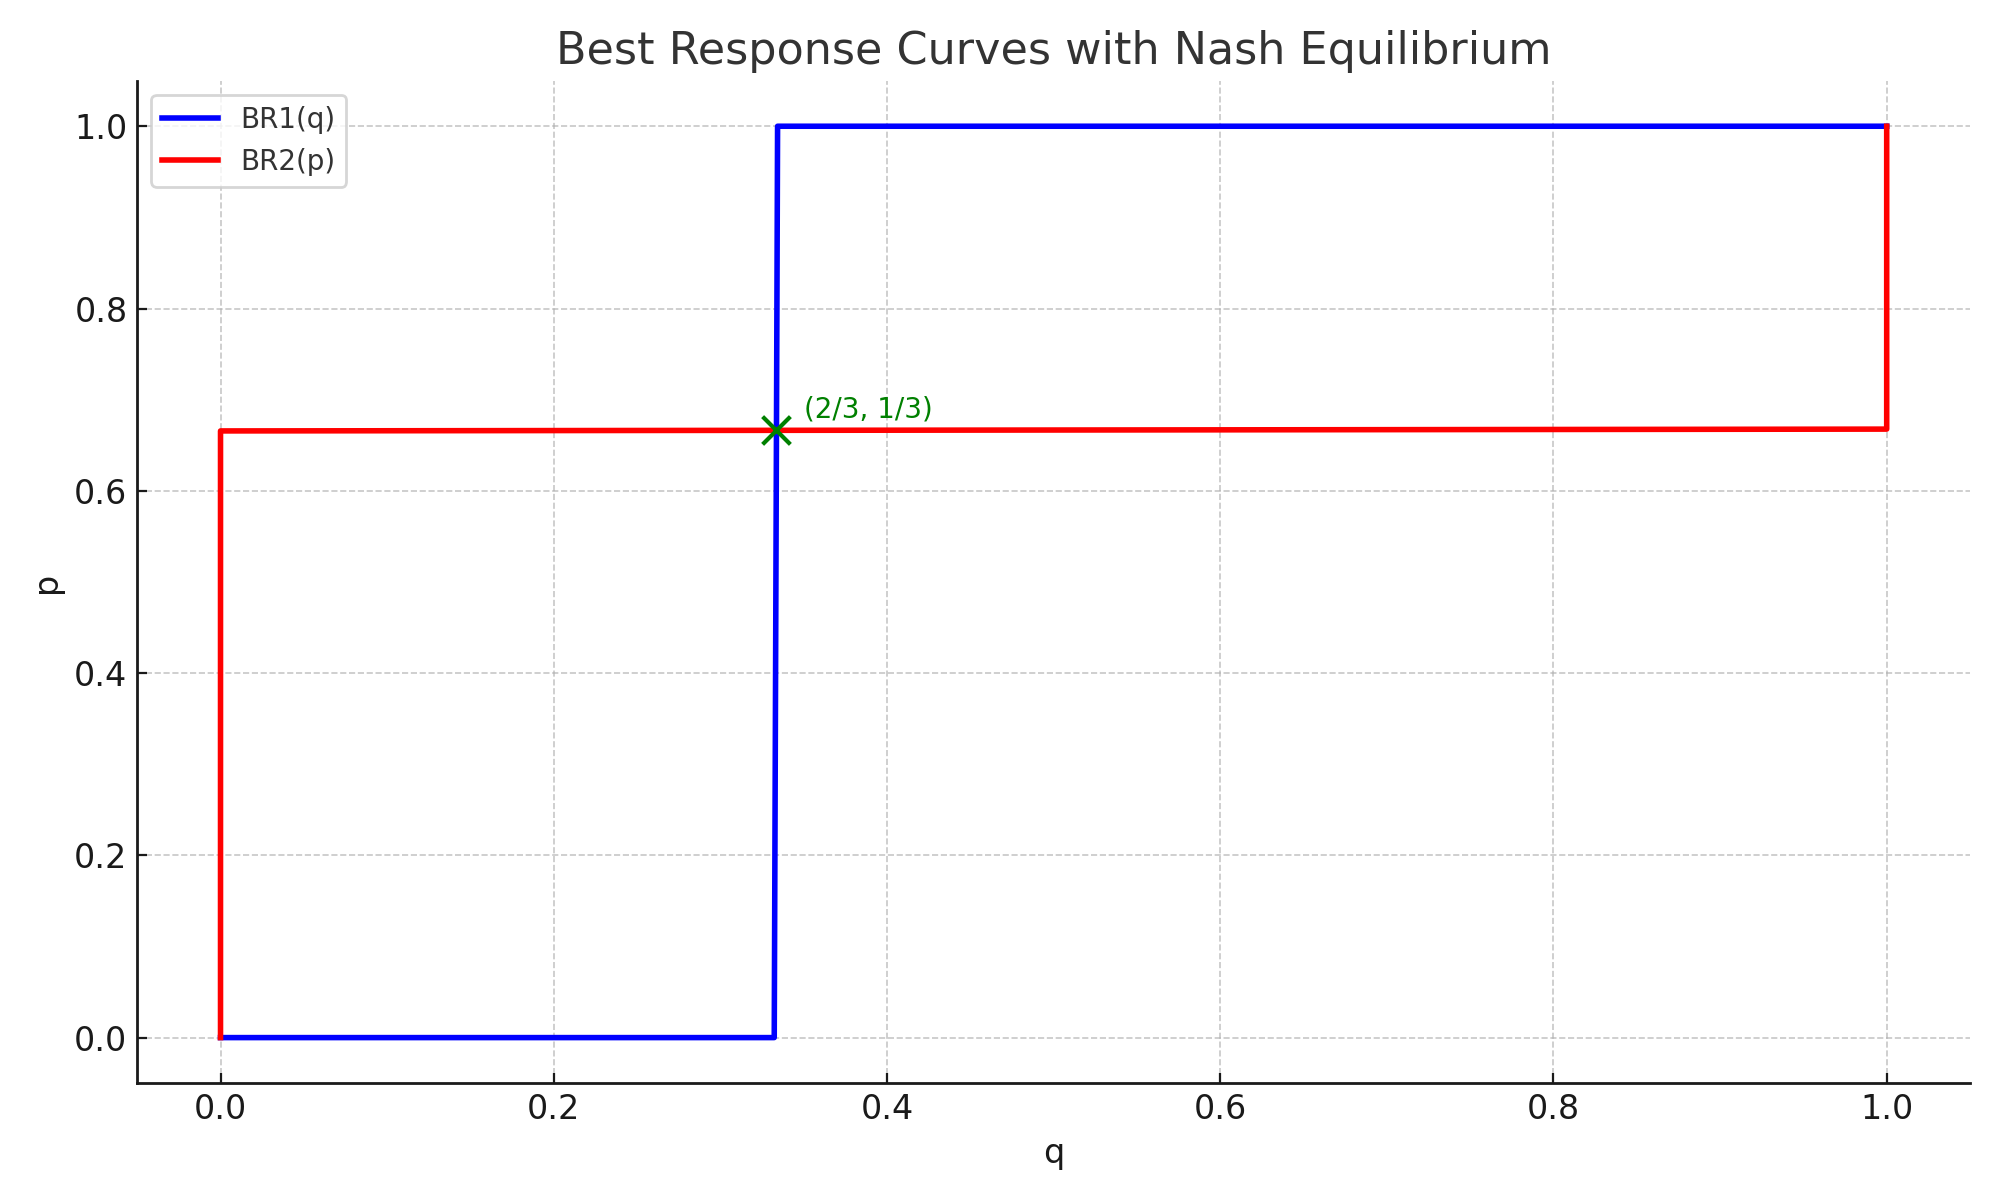
\includegraphics[width=0.95\textwidth]{./figures/best_response_curves1.png}
            \end{center}
            \caption{The best response for player 1 and player 2 given the other player's strategy. The point in the middle is the Nash equilibrium}\label{fig:resp1}
          \end{figure}

      \end{enumerate}

    \item
      \begin{enumerate}[label=(\roman*)]
        \item There are no dominant strategies and hence no dominant strategy equilibria. There are, however, two pure Nash equilibria given by $ (B, L) $ and $ (T, R) $.

        \item Both Nash equilibria maximize utilitarian social welfare and so are both Pareto optimal. However, only $ (B, L) $ maximizes egalitarian social welfare.

        \item Using the same two equations as before we get that the first equation turns into
          \begin{align*}
            0 \cdot q + 3 \cdot (1 - q) &= 4 \cdot q + 0 \cdot (1 - q) \\
            3 - 3q &= 4q \\
            q &= \frac{3}{7}
          \end{align*}
          while the second equation gives
          \begin{align*}
            0 \cdot p + 4 \cdot(1-p) &= 5\cdot p + 3 \cdot (1 - p) \\
            4 - 4p &= 5p + 3 - 3p \\
            p &= \frac{1}{6}.
          \end{align*}
          We thus have a fully mixed Nash equilibrium given by $ (\frac{1}{6}, \frac{3}{7}) $.

        \item Computing the utilities, we get
          \begin{align*}
            EU_1 \left( \frac{1}{6}, \frac{3}{7} \right) &= 3 \cdot \frac{1}{6}\cdot \frac{4}{7} + 4\cdot \frac{5}{6} \cdot \frac{3}{7} = \frac{12}{7}\\
            EU_2 \left( \frac{3}{7}, \frac{1}{6} \right) &= 5 \cdot \frac{1}{6} \cdot \frac{4}{7} + 4 \cdot \frac{5}{6}\cdot \frac{3}{7} + 3 \cdot \frac{5}{6}\cdot \frac{4}{7} = \frac{7}{3}
          .\end{align*}

        \item Since the Nash equilibrium is $ (p, q) = \left( \frac{1}{6}, \frac{3}{7} \right) $ we have the following best response functions
          \begin{align*}
            BR_1(q) &=
            \begin{cases}
              \{0\}, &\text{ if } q < \frac{3}{7}\\
              [0, 1], &\text{ if } q = \frac{3}{7}\\
              \{1\}, &\text{ if } q > \frac{3}{7}
            \end{cases} \\
            BR_2(p) &=
            \begin{cases}
              \{0\}, &\text{ if } p < \frac{1}{6}\\
              [0, 1], &\text{ if } p = \frac{1}{6} \\
              \{1\}, &\text{ if } p > \frac{1}{6}
            \end{cases}
          \end{align*}
          from which we get the plot:
          \begin{figure}[H]
            \begin{center}
              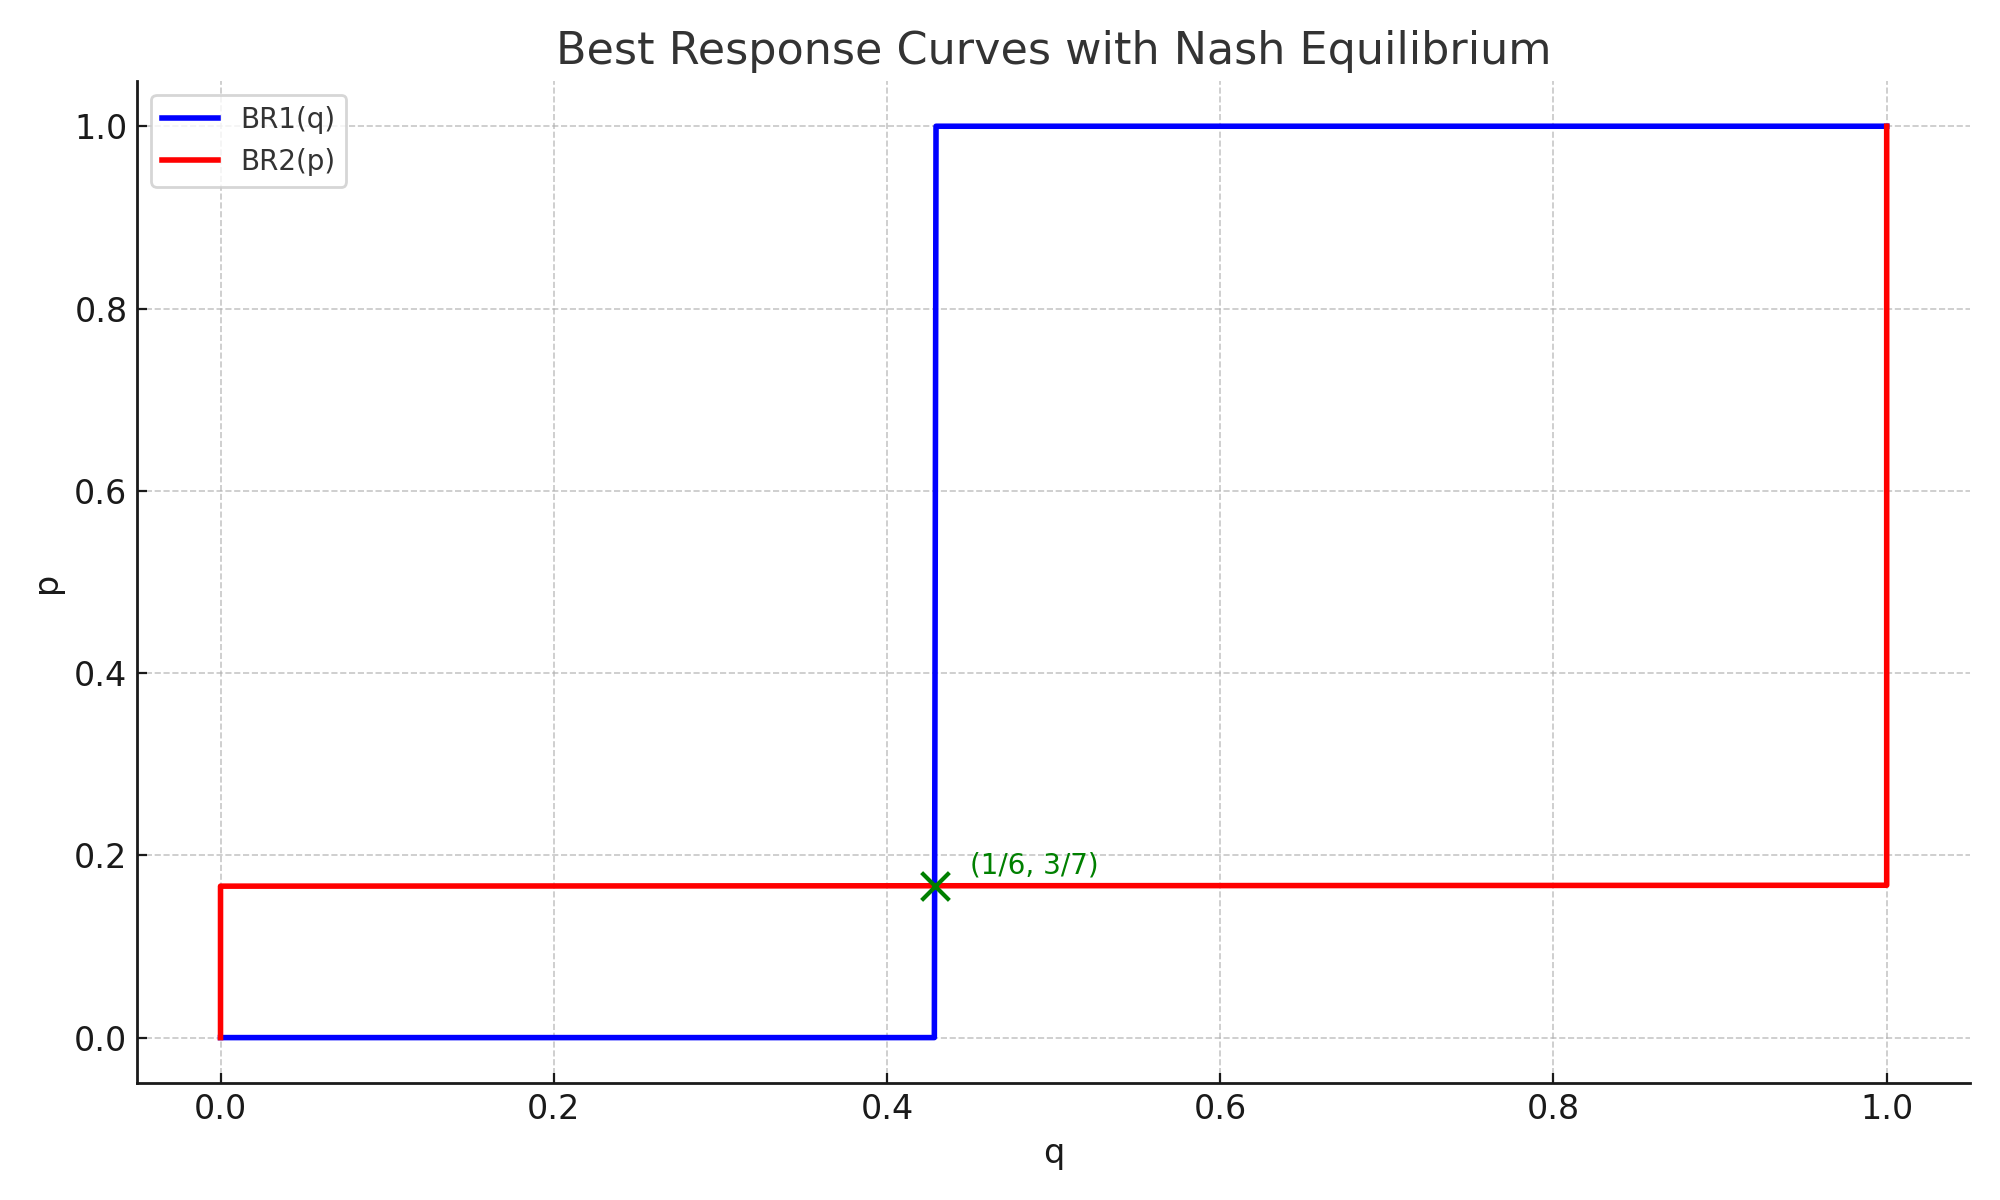
\includegraphics[width=0.95\textwidth]{./figures/best_response_curves2.png}
            \end{center}
            \caption{The best response for player 1 and player 2 given the other player's strategy. The point in the middle is the Nash equilibrium}\label{fig:resp2}
          \end{figure}

      \end{enumerate}
  \end{enumerate}
\end{exercise}

\begin{exercise}{4}
  There are two directions to prove.

  ($ \implies $): Assume that $ (p,q ) \in (0, 1)^2 $ is a fully mixed strategy Nash equilibrium in the generic $ 2 \times 2 $ game. We can without loss of generality focus on the first equation. To see why it must hold, consider the fact that
  \begin{equation*}
  EU_1(p,q) = p EU_1(T, q) + (1 - p) EU_1(B, q)
  .\end{equation*}
  If either $ EU_1(T, q) > EU_1(B, q) $ or $ EU_1(T, q) < EU_1(B, q) $ then player $ 1 $ would be better off choosing a pure strategy $ T $ or $ U $. Hence to satisfy the requirement that $ (p, q) $ is fully mixed Nash equilibrium we must have that $ EU_1(T, q) = EU_1(B, q) $.

  ($ \impliedby $): Assume the two equations hold. Considering again the equation
  \begin{equation*}
  EU_1(p,q) = p EU_1(T, q) + (1 - p) EU_1(B, q)
  \end{equation*}
  we see that this must imply $ (p, q) $ is a Nash equilibrium since there is no way for player $ 1 $ to alter his strategy so that the expected utility gets strictly higher. No matter what value he chooses for $ p $ the expected utility will always be the same and so he has no reason to deviate from his current strategy.
\end{exercise}

\begin{exercise}{5}
  \begin{enumerate}[label=(\alph*)]
    \item If we suppose that the utility function for both firms is simply the profit then we can describe this setting by the following $ 2 $-player payoff matrix:
      \begin{table}[H]
        \setlength{\extrarowheight}{2pt}
        \centering
        \begin{tabular}{*{4}{c|}}
          \multicolumn{2}{c}{} & \multicolumn{2}{c}{Player $Y$}\\\cline{3-4}
          \multicolumn{1}{c}{} &  & Buy  & Not Buy \\\cline{2-4}
          \multirow{2}*{Player $X$}  & Buy & $(\frac{2+n}{6 + 2n} - \frac{P}{2}, \frac{4+n}{6 + 2n} - \frac{P}{2})$ & $(\frac{1+n}{3+n} - P, \frac{2}{3 + n})$ \\\cline{2-4}
                                     & Not Buy & $(\frac{1}{3 + n}, \frac{2 + n}{3 + n} - P)$ & $(\frac{1}{3}, \frac{2}{3})$ \\\cline{2-4}
        \end{tabular}
      \end{table}

    \item If $ Buy $ is to be a weakly dominant strategy for firm $ X $ then we need that
      \begin{align*}
        u_X(\text{Buy}, \text{Buy}) &\geq u_X(\text{Not Buy}, \text{Buy}) \\
        u_X(\text{Buy}, \text{Not Buy}) &\geq u_X(\text{Not Buy}, \text{Not Buy})
      \end{align*}
      and in one of these cases the inequality needs to be strict. The two inequalities gives us the conditions
      \begin{align*}
        \frac{n}{3 + n} & \geq P \\
        \frac{2n}{9 + 3n} & \geq P.
      \end{align*}
      Hence, $ Buy $ is a weakly dominant strategy for $ X $ if $ P \leq 2n/(9+3n) $ since in this case we also get one strict inequality.

      Doing the same for player $ Y $ we have the two inequalities
      \begin{align*}
        u_Y(\text{Buy}, \text{Buy}) &\geq u_Y(\text{Buy}, \text{Not Buy}) \\
        u_Y(\text{Not Buy}, \text{Buy}) &\geq u_Y(\text{Not Buy}, \text{Not Buy})
      \end{align*}
      from which we get the requirements
      \begin{align*}
        \frac{n}{3+n} &\geq P \\
        \frac{n}{9+3n} &\geq P.
      \end{align*}
      Thus, $ Buy $ is a weakly dominant strategy for $ Y $ if $ P \leq \frac{n}{9+3n} $.

    \item For $ (Buy, Buy) $ to be a Nash equilibrium we need that
      \begin{align*}
        u_X(\text{Buy}, \text{Buy}) &\geq u_X(\text{Not Buy}, \text{Buy}) \\
        u_Y(\text{Buy}, \text{Buy}) &\geq u_X(\text{Buy}, \text{Not Buy}) \\
      \end{align*}
      which gives
      \begin{align*}
        \frac{n}{3 + n} &\geq P \\
        \frac{n}{3 + n} &\geq P.
      \end{align*}
      Hence $ (Buy, Buy) $ is a Nash equilibrium iff $ P \leq n/(3 + n) $.

    \item Similarly, for $ (Not\,\, Buy, Not\,\, Buy) $ to be a Nash equilibrium. We have the two inequalities
      \begin{align*}
        u_X(\text{Not Buy}, \text{Not Buy}) &\geq u_X(\text{Buy}, \text{Not Buy}) \\
        u_Y(\text{Not Buy}, \text{Not Buy}) &\geq u_Y(\text{Not Buy}, \text{Buy})
      \end{align*}
      which gives
      \begin{align*}
        P &\geq \frac{2n}{9 + 3n} \\
        P &\geq \frac{n}{9 + 3n}
      \end{align*}
      and so we have a Nash equilibrium for $ (Not\,\,Buy, Not\,\,Buy) $ when $ P \geq 2n/(9+3n) $.

    \item For $ (Buy, Not\,\, Buy) $ we have the inequalities
      \begin{align*}
        u_X(\text{Buy}, \text{Not Buy}) &\geq u_X(\text{Not Buy}, \text{Not Buy}) \\
        u_Y(\text{Buy}, \text{Not Buy}) &\geq u_Y(\text{Buy}, \text{Buy})
      \end{align*}
      which gives
      \begin{align*}
        \frac{2n}{9 + 3n} &\geq P \\
        \frac{n}{3 + n} &\leq P
      .\end{align*}
      Thus there can be no Nash equilibrium for $ (Buy, Not\,\,Buy) $. Similarly, for $ (Not\,\,Buy, Buy) $ there are inequalities
      \begin{align*}
        u_X(\text{Not Buy}, \text{Buy}) &\geq u_X(\text{Buy}, \text{Buy}) \\
        u_Y(\text{Not Buy}, \text{Buy}) &\geq u_Y(\text{Not Buy}, \text{Not Buy})
      \end{align*}
      which gives
      \begin{align*}
        \frac{n}{3+n} &\leq P \\
        \frac{n}{9 + 3n} &\geq P.
      \end{align*}
      Hence there is also no Nash equilibrium for $ (Not\,\,Buy, Buy) $.
  \end{enumerate}
\end{exercise}
\end{document}
